%! Suppress = MultipleIncludes
\documentclass[tikz,crop]{standalone}

% Part of the preamble, for TikZ figures.
% This is used in both the main document and in the subfigures.
% One exception is minted: since the path depends on the file, it is not set.
\usepackage{tikz}
\usepackage{xcolor}
\usepackage{pgfplots}

\pgfplotsset{compat=1.18}
\usepgfplotslibrary{statistics}

\usetikzlibrary{shapes,arrows,positioning,backgrounds,calc,intersections,calc}

\definecolor{ugent-re}{RGB}{220, 78, 40}        % vermilion			/ vermiljoen
\definecolor{ugent-we}{RGB}{45, 140, 168}       % no match
\definecolor{ugent-ge}{RGB}{232, 94, 113}       % rose				/ bleekrood
\definecolor{ugent-ea}{RGB}{111, 113, 185}      % distant blue		/ verblauw
\definecolor{ugent-pp}{RGB}{251, 126, 58}       % deep orange		/ dieporanje
\definecolor{ugent-ps}{RGB}{113, 168, 96}       % yellow green		/ geelgroen

\tikzstyle{python}=[fill=ugent-ps!50!white]
\tikzstyle{java}=[fill=ugent-we!50!white]
\tikzstyle{haskell}=[fill=ugent-ea!50!white]
\tikzstyle{js}=[fill=ugent-pp!50!white]
\tikzstyle{c}=[fill=ugent-re!50!white]

\newlength{\block}
\setlength{\block}{0.75cm}

\tikzstyle{a}=[anchor=north west]
\tikzstyle{box}=[a,draw,rectangle]
\tikzstyle{node}=[a,draw,minimum height=0.5cm,align=center,fill=white,text depth=.25ex]
\tikzstyle{document}=[node,tape,tape bend top=none]
\tikzstyle{cont}=[box,minimum height=1\block,minimum width=1\block]
\tikzstyle{arrow}=[draw, -latex]
\tikzstyle{inner}=[box,draw=gray]

% Blue box style
\tikzstyle{bluebox}=[draw=ugent-we,java]
\tikzstyle{redbox}=[draw=ugent-re,c]
\tikzstyle{greenbox}=[draw=ugent-ps,python]

% Some things specific to TESTed imagery.
\tikzstyle{tc}=[box,draw=ugent-ps]
\tikzstyle{comp}=[box,draw=ugent-re,fill=ugent-re,fill opacity=0.05]
\tikzstyle{exec}=[box,draw=ugent-we,fill=ugent-we,fill opacity=0.10]

% Stuff from tested-engine/concept.tex
\tikzstyle{process}=[node,rectangle]
\tikzstyle{terminator}=[node,rectangle,rounded corners=0.5cm]
\tikzstyle{io}=[node,trapezium,trapezium left angle=70,trapezium right angle=-70,minimum width=2.5cm,trapezium stretches=true]
\tikzstyle{small}=[font=\footnotesize,color=darkgray]
\tikzstyle{submission}=[document,align=right,minimum width=3cm,minimum height=1cm,text depth=0.5cm,inner sep=0.5mm,font=\scriptsize]

% Stuff from chatper3/flow.tex
\tikzstyle{height}=[minimum height=0.75\block]
\tikzstyle{contt}=[cont,minimum height=0.75\block]
\tikzstyle{compop}=[comp,text opacity=1]
\tikzstyle{execop}=[exec,text opacity=1]

\tikzstyle{hnode}=[draw,anchor=center,minimum height=\block,text depth=.25ex,align=center]
\tikzstyle{executable}=[hnode,ultra thick,fill=gray!10]
\tikzstyle{inner-exec}=[node,anchor=center,minimum width=3.25\block,densely dotted,font=\footnotesize,fill=none]
\tikzstyle{stmt}=[node,anchor=center,fill=gray!30,minimum width=4.5\block,font=\footnotesize]
\tikzstyle{fieldset}=[minimum height=\block,fill=white,text depth=.5ex,fill=white]

% Minted environments for use in Tikz
\newminted[tikzjava]{java}{autogobble,linenos=false,fontsize=\tiny,stripall}
\newminted[tikzpython]{python}{autogobble,linenos=false,fontsize=\tiny,stripall}
\newminted[tikztext]{text}{autogobble,linenos=false,fontsize=\tiny,stripall}


\begin{document}

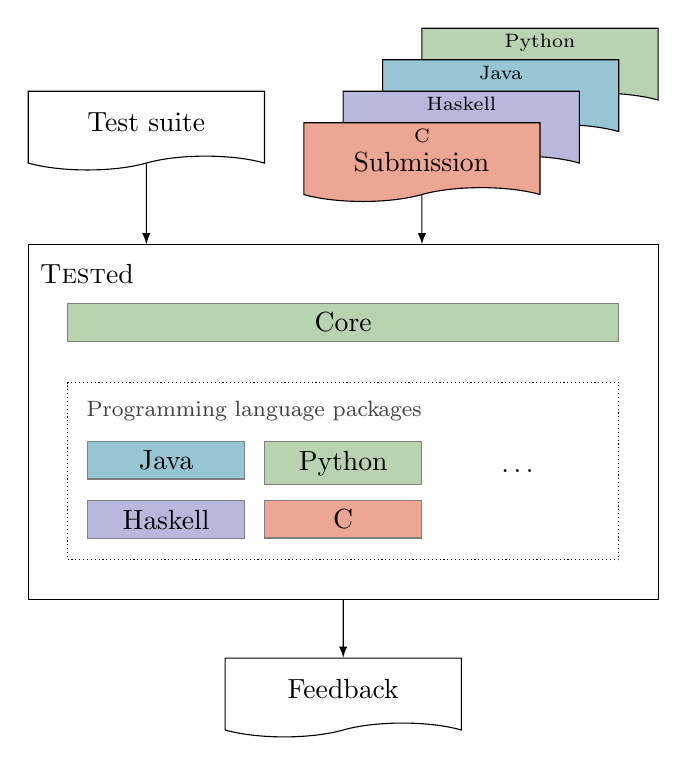
\begin{tikzpicture}
%    \draw[step=1.0,gray,thin] (0,0) grid (6,-16);

    \node[document,minimum width=3cm,minimum height=1cm] at (0, -0.8) (testplan) {Test suite};

    \node[submission,python] at (5, 0) (pysub) {Python};
    \node[submission,java] at (4.5, -0.4) (javasub) {Java};
    \node[submission,haskell] at (4, -0.8) (hssub) {Haskell};
    \node[submission,c] at (3.5, -1.2) (csub) {C};
    \node at (5, -1.7) (subm) {Submission};

    \node[process, minimum width=8cm, minimum height=4.5cm] at (0,-2.75) (tested) {};

    \draw[arrow] (csub) -- (tested.north-|csub);
    \draw[arrow] (testplan) -- (tested.north-|testplan);

    \node at (0.75, -3.125) (label) {\textsc{Test}ed};

    \node[inner, python, minimum width=7cm] at (0.5,-3.5) (core) {Core};
    \node[process, densely dotted, minimum width=7cm, minimum height=2.25cm] at (0.5,-4.5) (modules) {};
    \node[a,small] at (0.625, -4.625) (labelmod) {Programming language packages};
    \node[inner, java, minimum width=2cm] at (0.75,-5.25) (java) {Java};
    \node[inner, python, minimum width=2cm] at (3,-5.25) (python) {Python};

    \node[inner, haskell, minimum width=2cm] at (0.75,-6) (haskell) {Haskell};
    \node[inner, c, minimum width=2cm] at (3,-6) (c) {C};

    \node at (6.25,-5.625) (c) {\ldots};

    \node[document,minimum width=3cm,minimum height=1cm] at (2.5,-8) (feedback) {Feedback};

    \draw[arrow] (tested) -- (feedback);
\end{tikzpicture}

\end{document}
